


\chapter{绪论}
本章首先阐述了本文研究问题提出的背景,并总结了前人的工作以及该研究方向的难点和重点,以此提出了自己研究的具体任务,最后简要介绍了本文的内容框架。

\section{研究背景}
过去的十到二十年以来,在计算机视觉领域很大比例的文章都与人物相关,包括人体检测与跟踪、人脸识别、人体姿态或动作的识别等等。前两个研究方向相对较为成熟,现在的算法已经可以很容易做到实时同时正确率超过90\%,然而人体姿态的识别却一直未能攻克。人们在图像中表达的信息很大程度上是由其姿态(即动作)决定的,因此人体姿态识别具有很广阔的应用前景,在人机交互、影视动画、临床运动诊断、体育运动动作分析等方面都有重要应用价值。例如微软公司设计的kinect传感器就可以实时捕捉识别人体的三维姿态,成功地应用于人机交互游戏中。

目前,最为流行且实用的人体姿态捕捉方法是利用多台摄像机、在目标人物身上附加标记点或传感器,这种方法在电影特效、游戏动画等领域应用十分普遍,被公认为是最有效的方法。这种方法的最大优点就是姿态能够准确获得,但它的问题有很多,使得该方法的应用受到了限制。基于标记点的方法对硬件设备依赖较大,标记点处理复杂,传感器价格昂贵,且无法对已有的图像或视频进行分析。因此,目前的研究都是为了摆脱标记点,用人工智能的方法自动检测识别人体姿态。本文也顺应该研究方向,力求提高识别精度。

\section{研究现状}
\subsection{综述}
人体姿态识别的研究内容有很多种分类方式,首先我们根据姿态描述信息的多少分为姿态估计和动作分类两种,动作分类的任务是给定一张静止图像或图像序列,判定这张图片中人物的动作类比,例如wang等人~\cite{wang2007semi}只需要分辨图像中人的动作是拳击、跑步或鼓掌等动作即可,而姿态估计则需要给出人物的关节点的具体位置来描述姿态,包含了更丰富的信息,以下将着重介绍姿态估计的相关研究。还有一种分类方式是依据是否需要人工参与分为全自动和半自动估计,wei等人~\cite{wei2009modeling}~\cite{wei2010videomocap}的工作就是在人工标定一些关键帧后由算法估计出其他视频帧中的任务姿态,以下的介绍将集中于全自动估计方法。此外还可以根据使用的图像视角的数量分为单目识别和多目识别,在二维姿态估计中只需要单目图像信息,三维姿态估计则通常需要多目信息,如~\cite{bo2008fast}~\cite{burenius20133d}~\cite{bo2010twin}~\cite{Poppe2007},但也有单目估计的算法,如~\cite{wei2009modeling}~\cite{wei2010videomocap}~\cite{agarwal2006recovering}。此外还可以分为单人和多人识别、二维和三维估计等。
\subsection{二维姿态估计算法}
\subsubsection{基于生成模型的姿态估计算法}
理想的生成模型应该能考虑到姿态、衣着的多样性,从而能生成更真实的样本,然而由于复杂度限制,这是不可能实现的。因此,人们做了很多假设,将场景限定在一定的范围内,缩小了样本空间。这类方法事先通过统计等方法给出一个人体姿态分布的先验函数,然后用似然函数描述观察到的图片所含姿态与先验函数姿态的一致性。这种方法的效果好坏很大程度上依赖于先验函数的优劣。

\subsubsection{基于判别模型的姿态估计算法}
判别模型方法不是事先给定先验函数,而是直接学习后验分布,这种方法与生成模型相比更加快捷、易于实现~\cite{gkiox2013ariarticulated}。

\subsubsection{基于肢体的姿态估计算法}
这种方法将身体分为各个部分,所有的肢体(如头、胳膊、腿等)构成一个集合,因此对完整姿态的估计从一个高维模型化简为若干个低维的推断问题,同样,为了使数学推断更行之有效,~\cite{felzenszwalb2005pictorial}~\cite{ferrari2008progressive}~\cite{ramanan2007learning} 做了一些简化和假设。多数基于肢体的方法本质上也是生成模型,但通常也包含了判别模型~\cite{andriluka2009pictorial}。\cite{yang2011articulated}取得了非常好的结果。

\subsubsection{其他算法}
Wang等人~\cite{wang2013beyond}使用了一种隐含树模型,通过学习各肢体间的关系,构建出一个树结构的图模型,在LSP~\cite{Johnson10LSP} 和PARSE~\cite{ramanan2007learning}数据集上得到了目前最优秀的结果。Tian等人~\cite{tian2012exploring}也使用了一种类似的树形结构,将人体分为三层,并用离散的类别刻画局部动作,取得了几乎是最好的结果。

\subsection{三维姿态估计算法}
\subsubsection{基于特征的姿态估计算法}
基于特征的方法本质上是基于判别模型的方法~\cite{agarwal2006local}~\cite{rosales2002learning}~\cite{shakhnarovich2003fast}~\cite{sminchisescu2005discriminative},输入图像被抽象成特征描述,经过学习得到模型,从而进行预测。代表性的几种方法有:Sminchisescu等人的SSLVM~\cite{bo2009SSLVM}、条件混合专家预测~\cite{bo2008fast}、双高斯过程~\cite{bo2010twin}。

\subsubsection{基于二维姿态估计的算法}
这种算法~\cite{burenius20133d}不关心二维姿态的估计,算法假定多视角的二维姿态已知,通过数据融合,推算出三维姿态,其强调的是如何将已有的二维姿态融合推广至三维情况。

\subsubsection{半自动姿态估计算法}
该算法~\cite{wei2009modeling}~\cite{wei2010videomocap}已在前文介绍,不再赘述。

\subsection{研究难点}
相关研究之所以未能取得很大突破,究其原因主要有如下几点,这些因素被公认为人体姿态估计领域的重要挑战。
\begin{enumerate}[(1)]
  \item 图像中人物外貌、衣着的多样性
  \item 光照条件的多样性
  \item 遮挡问题,包括自身肢体遮挡、他人或场景中物品对人物的遮挡
  \item 人体骨架的复杂性
  \item 人体姿态是一个高维描述
  \item \label{itm:3D}图片中丢失了3D信息
  \item 复杂的背景环境
\end{enumerate}
其中(\ref{itm:3D})在多目估计中不存在,因此多目图像估计能够更好地克服遮挡等问题。

\section{问题描述}
本文将研究内容聚焦于人体三维姿态的估计,具体说来,输入与输出如下:
\begin{description}
  \item[输入] 无标记的单目或多目静止图像(可以推广至图像序列)
  \item[输出] 用关节点表示的三维人体骨架(关于骨架表示法将在\ref{sec:skeleton}阐述)
\end{description}

可以参照图\ref{fig:inout}。

\begin{figure}[htbp]
    \centering
    \subcaptionbox{输入}{
    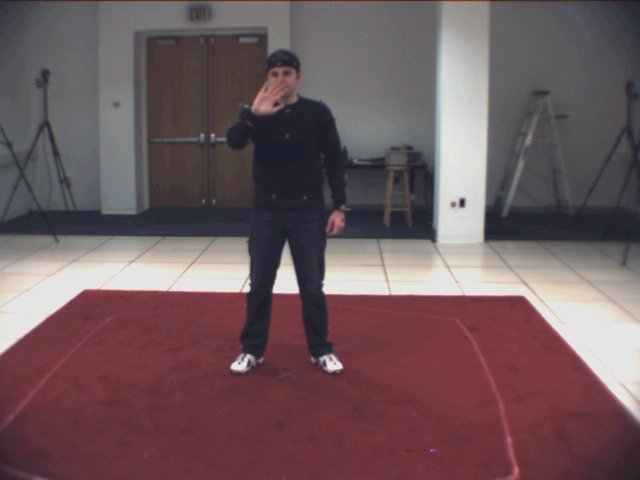
\includegraphics[height=6cm]{humaneva1.png}}
    \hspace{2cm}
    \subcaptionbox{输出}{
    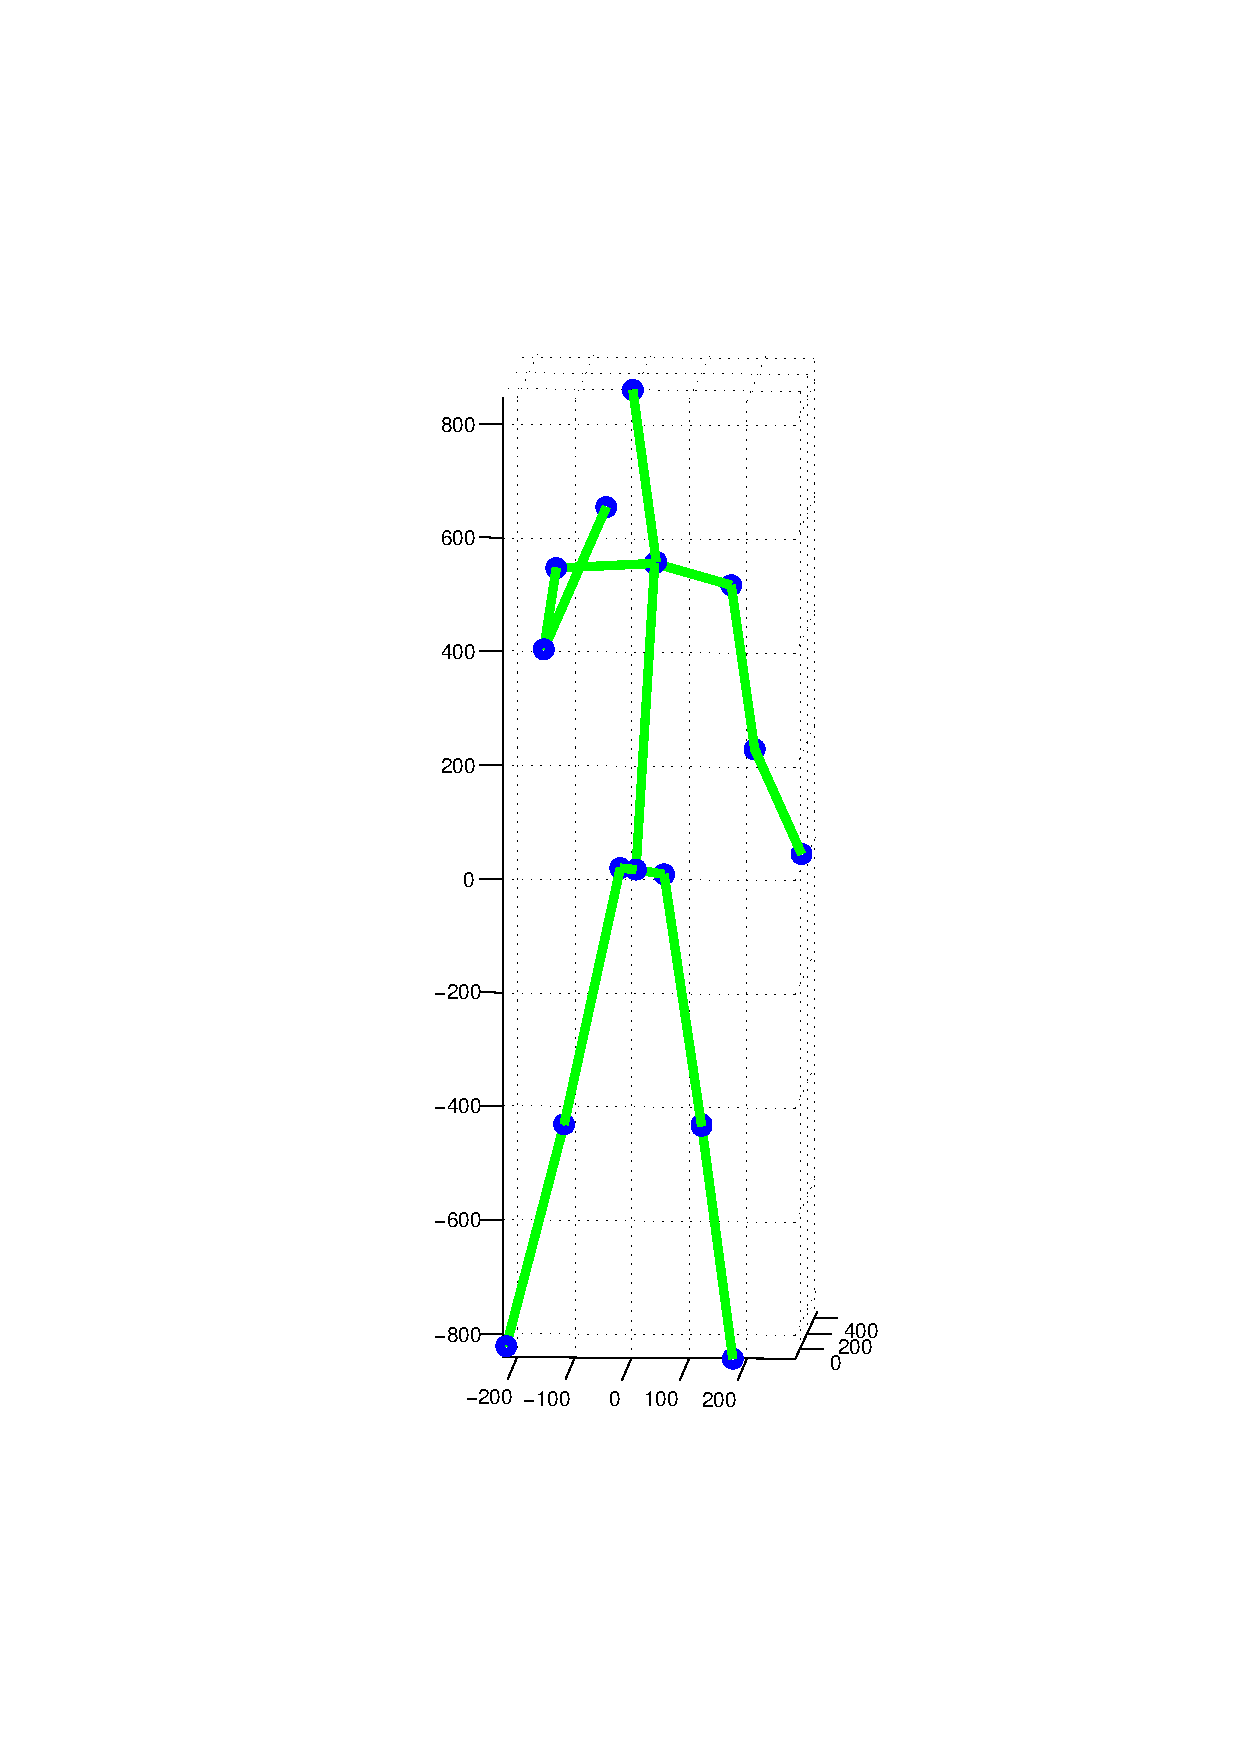
\includegraphics[height=6cm]{humaneva1_bone.pdf}}
    \caption{本文研究问题的输入与输出}
    \label{fig:inout}
\end{figure}


\section{文章结构}
本文共分为六章,第二章将介绍本人研究工作所依赖的数据库,包括数据库的内容、统计信息以及如何利用数据库等,其次介绍了本文所用的人体骨架模型的表示方法。第三章将介绍特征提取的一些方法,以及本文采用的特征以及其表示方法。第四章详细介绍了姿态估计算法,该算法基于双高斯过程,较好地考虑了输入输出变量之间的耦合关系。第五章主要以图表的方式整理了所做工作的结果,通过与前人工作对比,证明了本文工作的意义,并从结果中发现总结问题,分析可能的原因。第六章对全文做以总结,最后针对还存在的问题提出一些可能的解决方法和未来的努力方向。
